%%%%%%%%%%%%%%%%%%%%%%%%%%%%%%%%%%%%%%%%%
% Beamer Presentation
% LaTeX Template
% Version 1.0 (10/11/12)
%
% This template has been downloaded from:
% http://www.LaTeXTemplates.com
%
% License:
% CC BY-NC-SA 3.0 (http://creativecommons.org/licenses/by-nc-sa/3.0/)
%
%%%%%%%%%%%%%%%%%%%%%%%%%%%%%%%%%%%%%%%%%

%----------------------------------------------------------------------------------------
%	PACKAGES AND THEMES
%----------------------------------------------------------------------------------------

\documentclass{beamer}
\usepackage{amsmath, amssymb}

\usepackage{bm}

\mode<presentation> {

% The Beamer class comes with a number of default slide themes
% which change the colors and layouts of slides. Below this is a list
% of all the themes, uncomment each in turn to see what they look like.

%\usetheme{default}
%\usetheme{AnnArbor}
%\usetheme{Antibes}
%\usetheme{Bergen}
%\usetheme{Berkeley}
%\usetheme{Berlin}
%\usetheme{Boadilla}
\usetheme{CambridgeUS}
%\usetheme{Copenhagen}
%\usetheme{Darmstadt}
%\usetheme{Dresden}
%\usetheme{Frankfurt}
%\usetheme{Goettingen}
%\usetheme{Hannover}
%\usetheme{Ilmenau}
%\usetheme{JuanLesPins}
%\usetheme{Luebeck}
%\usetheme{Madrid}
%\usetheme{Malmoe}
%\usetheme{Marburg}
%\usetheme{Montpellier}
%\usetheme{PaloAlto}
%\usetheme{Pittsburgh}
%\usetheme{Rochester}
%\usetheme{Singapore}
%\usetheme{Szeged}
%\usetheme{Warsaw}

% As well as themes, the Beamer class has a number of color themes
% for any slide theme. Uncomment each of these in turn to see how it
% changes the colors of your current slide theme.

%\usecolortheme{albatross}
%\usecolortheme{beaver}
%\usecolortheme{beetle}
%\usecolortheme{crane}
%\usecolortheme{dolphin}
%\usecolortheme{dove}
%\usecolortheme{fly}
%\usecolortheme{lily}
%\usecolortheme{orchid}
\usecolortheme{rose}
%\usecolortheme{seagull}
%\usecolortheme{seahorse}
%\usecolortheme{whale}
%\usecolortheme{wolverine}

%\setbeamertemplate{footline} % To remove the footer line in all slides uncomment this line
%\setbeamertemplate{footline}[page number] % To replace the footer line in all slides with a simple slide count uncomment this line

%\setbeamertemplate{navigation symbols}{} % To remove the navigation symbols from the bottom of all slides uncomment this line
}

\usepackage{graphicx} % Allows including images
\usepackage{booktabs} % Allows the use of \toprule, \midrule and \bottomrule in tables

%----------------------------------------------------------------------------------------
%	TITLE PAGE
%----------------------------------------------------------------------------------------

\title[Pima Indians]{Predicting Diabetes in  Pima Indian Women} % The short title appears at the bottom of every slide, the full title is only on the title page

\author{Nik Po\v cu\v ca} % Your name
\institute[McMaster University] % Your institution as it will appear on the bottom of every slide, may be shorthand to save space
{
McMaster University \\ % Your institution for the title page
\medskip
\textit{Data Science 780} % Your email address
}
\date{\today} % Date, can be changed to a custom date

\begin{document}

\begin{frame}
\titlepage % Print the title page as the first slide
\end{frame}

\begin{frame}
\frametitle{Overview} % Table of contents slide, comment this block out to remove it
\tableofcontents % Throughout your presentation, if you choose to use \section{} and \subsection{} commands, these will automatically be printed on this slide as an overview of your presentation
\end{frame}

%----------------------------------------------------------------------------------------
%	PRESENTATION SLIDES
%----------------------------------------------------------------------------------------

%------------------------------------------------
\section{Introduction} % Sections can be created in order to organize your presentation into discrete blocks, all sections and subsections are automatically printed in the table of contents as an overview of the talk
%------------------------------------------------

\begin{frame}
\frametitle{Future of Diabetes in Canada}
\begin{block}{What is diabetes?}
Diabetes is an ongoing chronic illness that causes the body to have an inability to process glucose (sugar) by restricting or eliminating the kidney's ability to produce insulin. 
\end{block}
\begin{block}{Rate of Diabetes}
By 2025 the estimated prevalence of diabetes in Canada will increase to 5 million individuals.
\end{block}
\begin{block}{Cost of Diabetes}
Cost alone is said to increase by $ 25 \%$ putting a strain on the system. 
\end{block}
\end{frame}

\begin{frame}
\frametitle{Introduction to the Pima Indian dataset}
The Pima Indians dataset contains a population of women who were at least 21 years old of Pima Indian heritage and living near Phoenix, Arizona (Smith et~al.1988).
\begin{itemize}
\item $ 532$ complete records
\item The population was tested for diabetes according to World Health Organization criteria.
\item The dataset contains $7$ covariates and $1$ response variable
\end{itemize}
\end{frame}
%------------------------------------------------


\begin{frame}{Description of covariates and response}
\begin{tiny}
\begin{minipage}{\textwidth}
\centering
\begin{tabular}{|llrrrr|}
\hline
Variable & Description & $\mu$ & $\sigma$ & min & max \\ 
\hline
$npreg$      & number of pregnancies (integer)                                                                                     & 3.52   & 3.31  & 0.00  & 17.00  \\
$glu$   & plasma glucose concentration. (integer)\footnote{count of quantity of plasma after 2 hours} & 121.03 & 30.97 & 56.00 & 199.00 \\
$bp$         & diastolic blood pressure (mm Hg).                                                                                   & 71.51  & 12.30 & 24.00 & 110.00 \\
$skin $      & triceps skin fold thickness (mm).                                                                                   & 29.18  & 10.51 & 7.00  & 99.00  \\
$bmi $       & body mass index (weight in kg/height in m$^2$).                                    & 32.89  & 6.87  & 18.20 & 67.10  \\
$ped$        & diabetes pedigree function \footnote{diabetes mellitus history in relatives and the genetic relationship of those relatives to the patient }                                                                               & 0.50   & 0.34  & 0.09  & 2.42   \\
$age$        & age in years. (integer)                                                                                             & 31.61  & 10.75 & 21.00 & 81.00  \\
\hline
$type $      & Yes or No (binary response)                                                & -      & -     & -     & -     \\
\hline
\end{tabular}
\end{minipage}
\end{tiny}
\end{frame}

%------------------------------------------------


\begin{frame}{Pair plot of covariates}
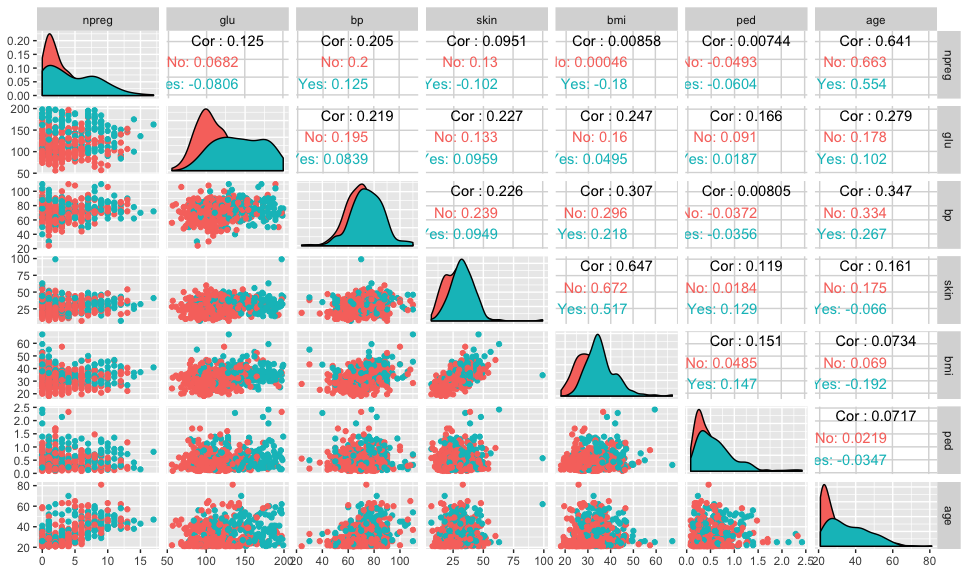
\includegraphics[scale=0.35]{plotgg}
\end{frame}

\section{Methodology}


\begin{frame}{Data Preperation}
\begin{itemize}
\item Due to differences in max and min, all of the covariates were scaled. 
\item An 80/20 - training/test split was constructed at random. 
\item A second training set was created by bootstrapping the first to have balanced diabetic and non-diabetic individuals.

\end{itemize}
\end{frame}


\begin{frame}{Methodological Overview}
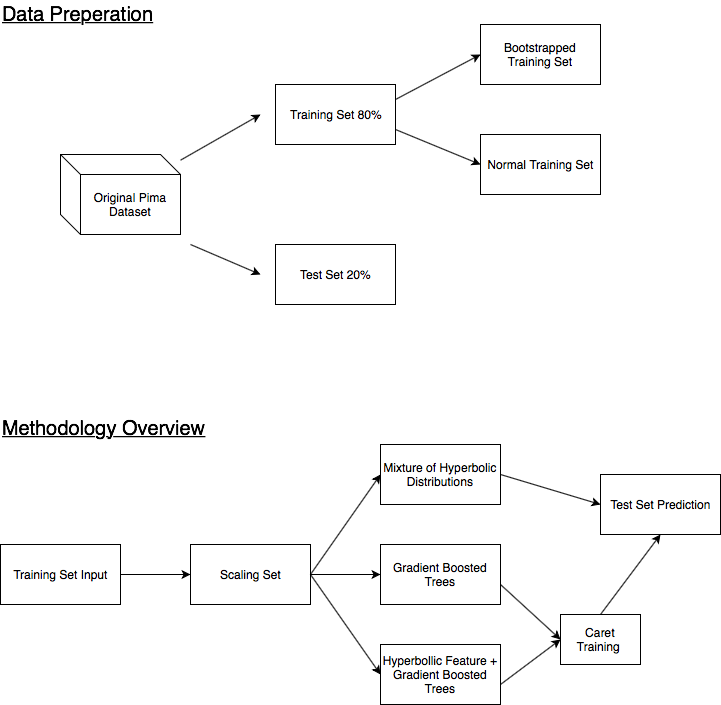
\includegraphics[scale=0.30]{MethodOverview}
\end{frame}

\begin{frame}{Mixtures of Generalized Hyperbolic Distributions (McNicholas P.D. 2015) }

Consider a random vector $\bm{X}$ that emanates from a finite mixture model with $\bm{x} \in \bm{X}$ with $\bm{x}$ as a realization of $ \bm{X}$. Furthermore assume that for the sample space $\Omega$, where $X \in \Omega$ one can partition $\Omega$ into $G$ subgroups $\Omega = \{\Omega_1, \dots ,\Omega_G \}$. Stemming from this the joint distribution of $\bm{X}$ is written as

$$f(\bm{x}| \bm{\theta}) = \sum_{g = 1}^G \pi_g f(\bm{x}| \bm{\theta}_g), $$


\end{frame}


\begin{frame}{Mixtures of Generalized Hyperbolic Distributions}
Given an assumption that $\bm{X}$ is of a generalized hyperbolic distribution (Tortora et. al 2014), then $f(\bm{x}| \bm{\theta}_g)$ is formulated as 
\begin{tiny}
$$ f (\bm{x}| \bm{\theta}_g) = \left[ \frac{ \omega_g + \delta(  \bm{x}, \bm{\mu_g} | \bm{\Sigma}_g  )     }{ \omega_g +  \alpha^{'}_g \bm{\Sigma^{-1}}_g \alpha_g  }\right]^{(\lambda - p/2)/2} \frac{K_{\lambda - p/2} \left( \sqrt{ (\omega_g +  \alpha^{'}_g \bm{\Sigma^{-1}}_g \alpha_g ) (  \omega_g + \delta(  \bm{x}, \bm{\mu_g} | \bm{\Sigma}_g  ))   }    \right)    }{(2 \pi)^{p/2} |\Sigma|^{1/2} K_\lambda(\omega_g) \exp\{ - ( \bm{x} - \bm{\mu}_g)^{'} \bm{\Sigma_g}^{-1} \bm{\alpha}_g\}  } .   $$ 
\end{tiny}
\end{frame}


\begin{frame}{Mixture Discriminant Analysis}

$$L(\bm{\theta}) =   \prod_{i=1}^k \sum_{g=1}^G \left[  \pi_g f(\bm{x}| \bm{\theta}_g) \right]^{z_{ig}} \times \prod_{j=k+1}^n \sum_{h=1}^H \left[\pi_h\phi(\bm{x}_j| \bm{\theta}_h) \right].$$


$$z_{jh} = \arg \max_{h \in H} \tau_{ih}  , \quad \tau_{ih} = \frac{\hat{\pi}_{ih}  f(\bm{x}| \bm{\theta}_h)  }{ \sum_{h=1}^H \hat{\pi}_{ih}  f(\bm{x}| \bm{\theta}_h) }. $$


\end{frame}


\begin{frame}{Gradient Boosted Trees}
Given a set of data with $n$ observations and $m$ covariates ($\bm{x_i}$) on some set $D = \{ (x_i,y_i) \}$. A tree ensemble uses $K$ additive functions to predict the output of ($y_i$) written as follows 
$$ \hat{y_i}  = \sum_{k=1}^K \lambda f_k(\bm{x}_i), $$ 

$$L^{(t)} = \sum_{i=1}^n l(y_i, \hat{y}^{(t-1)}_i + f_k(\bm{x}_i)) + \phi(f_k) $$

\end{frame}


\begin{frame}{Evaluation Methodology}
$$\textbf{BIC} = \log(n) k - 2 \log(\hat{L}), $$

$$ARI = \frac{ \sum_{ij} \binom{n_{ij}}{2} - [\sum_i \binom{a_i}{2} \sum_j \binom{b_j}{2}] / \binom{n}{2} }{ \frac{1}{2} [\sum_i \binom{a_i}{2} + \sum_j \binom{b_j}{2}] - [\sum_i \binom{a_i}{2} \sum_j \binom{b_j}{2}] / \binom{n}{2} }, $$
\end{frame}



\section{Results}

\begin{frame}{Training Results}
\begin{small}
\begin{table}[!h]
\centering
\caption{Model performance results with ARI and class error over all six variations. }
\vspace{5pt}
\label{modelPerf}
\begin{tabular}{|l|rr|}
\hline\hline
Method                                         & ARI    & Class Error \\
\hline
DA Hyperbolic                                  & 0.1974 & 0.2710      \\
DA Hyperbolic + Boostrap                       & 0.2203 & 0.2617      \\
Boosted Trees                                  & 0.3532 & 0.1963      \\
Boosted Trees + Boostrap                       & 0.3532 & 0.1963      \\
Boosted Trees + Hyperbolic Feature             & $\bm{0.3546}$ & $\bm{0.1963}  $   \\
Boosted Trees + Hyperbolic Feature + Bootstrap & 0.3546 & 0.1963     \\
\hline\hline
\end{tabular}
\end{table}
\end{small}
\end{frame}


\begin{frame}{Boosted Tree with Hyperbolic Features}
\begin{tiny}
\begin{table}
\label{classTable}
\caption{Classification table for mixture of hyperbolic distributions (left) and gradient boosted trees (right), vertical (0,1) is positive for diabetes and horizontal is mixture class label.}
\vspace{8pt}
\centering
\begin{tabular}{|r|rrrrr|}
\hline\hline
Classes & 1  & 2  & 3  & 4  & 5  \\
\hline
0       & 8  & 93 & 76 & 34 & 77 \\
1       & 17 & 20 & 54 & 31 & 15 \\ 
\hline \hline
\end{tabular}
$\quad\quad$
\begin{tabular}{|r|rr|}
\hline\hline
          & \underline{Predicted} &   \\
\underline{True Values} & 0         & 1  \\
\hline
0           & 64        & 3  \\
1           & 17        & 23 \\
\hline\hline
\end{tabular}
\end{table}

\begin{table}[!h]
\centering
\label{relInflu}
\caption{Relative influence of each covariate on boosted tree prediction in percetages. }
\vspace{5pt}
\begin{tabular}{|l|llllllll|}
\hline\hline 
Variable                & glu    & age    & bmi    & ped   & npreg & skin  & hyper & bp    \\ 
\hline
Relative Influence (\%) & 51.480 & 18.203 & 13.484 & 9.989 & 5.107 & 1.253 & 0.484 & 0.000  \\
\hline\hline
\end{tabular}
\end{table}
\end{tiny}
\end{frame}

\begin{frame}{Conclusions}
\begin{block}{Limitations}
Gradient boosted trees are limited in their predictive power when covariates do not necessarily predict response.
\end{block}
\begin{block}{Improvements}
Slight improvements can be made to model accuracy by using mixture models to generate sub groups for prediction.
\end{block}
\begin{block}{More Covariates}
This gradient boosted trees are not sufficient in predicting diabetes accurately and other types of data should be collected to improve predictive power. 
\end{block}
\end{frame}



\begin{frame}
\frametitle{References}
\footnotesize{
\begin{thebibliography}{99} % Beamer does not support BibTeX so references must be inserted manually as below
\begin{tiny}

\bibitem[{Chen and Guestrin(2016)}]{gradientboost}
Chen, T., Guestrin, C., 2016. Xgboost: {A} scalable tree boosting system. CoRR
  abs/1603.02754.
\newblock Scalable Tree Boosting

\bibitem[{Chubbs(2017)}]{diabetes}
Chubbs, D.~O., 2017. Primary Care Provider Adherence to the Canadian Diabetes
  Association Clinical Practice Guideline for Chronic Kidney Disease.
\newblock Clinical Practice Guideline for Kidney Disease


\bibitem[{Dempster et~al.(1977)Dempster, Laird, and Rubin}]{dempster}
Dempster, A.~P., Laird, N.~M., Rubin, D.~B., 1977. Maximum likelihood from
  incomplete data via the {EM}-algorithm. Journal of the Royal Statistical
  Society B 39, 1--38.
  \newblock Expectation Maximization Algorithm


\bibitem[{Max~Kuhn et~al.(2018)Max~Kuhn, Weston, Williams, Keefer, Engelhardt,
  Cooper, Mayer, Kenkel, the R~Core~Team, Benesty, Lescarbeau, Ziem, Scrucca,
  Tang, Candan, and Hunt.}]{caret}
Max~Kuhn, J.~W., Weston, S., Williams, A., Keefer, C., Engelhardt, A., Cooper,
  T., Mayer, Z., Kenkel, B., the R~Core~Team, Benesty, M., Lescarbeau, R.,
  Ziem, A., Scrucca, L., Tang, Y., Candan, C., Hunt., T., 2018. caret:
  Classification and Regression Training. R package version 6.0-80.
\newblock Caret Package

\bibitem[{McNicholas(2015)}]{mixdist}
McNicholas, P.~D., 2015. Mixture Model-Based Classification. Chapman and Hall.
\newblock Mixture Model-Based


\bibitem[{Smith et~al.(1988)Smith, Everhart, Dickson, Knowler, and
  Johannes}]{pima}
Smith, J.~W., Everhart, J.~E., Dickson, W.~C., Knowler, W.~C., Johannes, R.~S.,
  1988. Using the adap learning algorithm to forecast the onset of diabetes
  mellitus. In: Proceedings of the Annual Symposium on Computer Application in
  Medical Care. pp. 261--265.
  \newblock Pima Indian Dataset 

\bibitem[{{Tortora} et~al.(2014){Tortora}, {Franczak}, {Browne}, and
  {McNicholas}}]{hyper}
{Tortora}, C., {Franczak}, B.~C., {Browne}, R.~P., {McNicholas}, P.~D., Mar.
  2014. {A Mixture of Coalesced Generalized Hyperbolic Distributions}. ArXiv
  e-prints.
  \newblock Mixture of Coalesced Generalized Hyperbolic


\end{tiny}

\end{thebibliography}
}
\end{frame}

%------------------------------------------------

\begin{frame}
\Huge{\centerline{The End}}
\end{frame}

%----------------------------------------------------------------------------------------

\end{document}